\section{Concurrency}
\subsection{Motivation}
\subsubsection{Wieso wird Concurrency verwendet?}
\begin{itemize}
  \item Praktische Programme führen meist mehrere Arbeiten "`gleichzeitig"' aus. 
\end{itemize}
\subsubsection{Parallelität vs. Concurrent Computing}
\begin{itemize}
  \item Parallel Computing
  	\begin{itemize}
  	  \item execution of different tasks is really at the same time
  	  \item is not possible on a single-core machine 
  	\end{itemize}
  \item Concurrent Computing
  	\begin{itemize}
  	  \item execution of different tasks only seems to be at the same time
  	  \item different tasks get consecutive time slices
  	  \item there's only one task really running at a particular time slice
  	  \item can be done on a single- or multicore machine 
  	\end{itemize} 
\end{itemize}
\subsubsection{Gründe, Concurrency nicht zu verwenden}
\begin{itemize}
  \item Concurrency (mit Prozessen, Tasks, Threads) kostet immer
  \begin{itemize}
  	\item Stack
  	\item Context switch (Umschalten vom einen zum anderen) 
  	  \begin{itemize}
  	  \item dauert
  	  \item Alter Context muss gespeichert, neuer wieder geladen werden
  	  \end{itemize}
  	\item Zugriff auf gemeinsame Ressourcen muss synchronisiert werden 
  	  \begin{itemize}
  	  \item kostet
  	  \item fehleranfällig (wird vergessen oder falsch gemacht)
  	  \end{itemize}
  \end{itemize}
\item Komplexität steigt
  \begin{itemize}
  \item Sequentielle Programme sind einfacher zu verstehen als parallele
  \item Ziel ist immer, ein System möglichst einfach zu halten
  \end{itemize}
\end{itemize}

\textbf{Folgerung:} Concurrency nur dann einsetzen, wenn wirklich ein Nutzen vorhanden ist!

\subsection{POSIX Threads Programming}
\subsubsection{UNIX Process}
\begin{itemize}
\item Heavyweight process (created by the operating system)
\item Processes require a fair amount of overhead; they contain information about program resources and program execution state, including: Process ID, process group ID, user ID, and group ID; Enviroment; Program instructions; Registers; Stack; Heap; File descriptors; Signal actions; Shared libraries; Inter-process communication tools
\end{itemize}
\subsubsection{UNIX Thread}
\begin{itemize}
\item Lightweight "process"
\item Threads use and exist within the process resources
\item A thread uses the same address space as other threads of the same process
\item Threads are able to be scheduled by the operating system
\item Independent stream of instructions that may run simultaneously to other streams of instructions
\item Procedure that runs independently from its main program
\item A thread maintains its own: Stack pointer; Registers; Scheduling properties; Set of pending and blocked signals; Thread specific data
\item Concurrent programs are usually achieved with threads
\end{itemize}
\subsubsection{Process vs. Thread in UNIX}
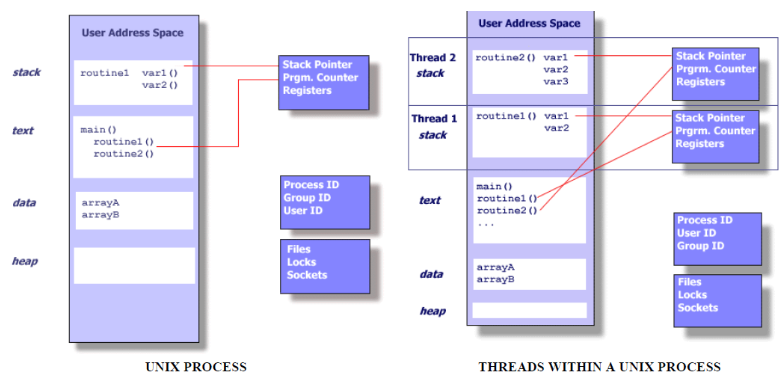
\includegraphics[width=12cm]{images/Concurrency/ProcessVsThread.png}\\\\
Man beachte: Alles was ein Thread inne hat, hat ein Prozess auch inne (aber NICHT umgekehrt)!
\subsubsection{What are POSIX Threads?}
\begin{itemize}
\item For UNIX systems, a standardized C language threads programming interface has been specified by the IEEE POSIX 1003.1c standard.
\item The short form of POSIX threads is Pthreads or pthreads.
\end{itemize}
\subsubsection{The pthreads API}
\begin{itemize}
\item Routines of the pthreads API start with pthread\_
\item The header file pthread.h must be included
\item The link command must include –lpthread
\end{itemize}
\subsubsection{Starting and Terminating a Thread}
\begin{itemize}
\item Any routine with the following interface may become a thread routine:\newline
\lstinline{void* threadRoutine(void* arg);}
\item A thread is started with:\newline
\lstinline{int pthread_create(pthread_t* thread, const pthread_attr_t* attr, void* (*startRoutine) (void*), void* arg);}
  \begin{itemize}
  \item thread: pointer to a pthread\_t instance
  \item attr: pointer to a pthread\_attr\_t structure, often 0 (default attributes)
  \item arg: a single argument that may be passed to startRoutine
  \item returns 0 on success 
  \end{itemize}
\item A thread terminates in one of the following ways:
  \begin{itemize}
  \item it calls pthread\_exit()
  \item it returns from startRoutine
  \item it is canceled with pthread\_cancel()
  \end{itemize}
\end{itemize}
\textbf{Example - Starting a Thread}
\lstinputlisting[style=C]{snippets/Threads/thread_start.c}
\textbf{Example - Waiting on a Thread to Finish}
\lstinputlisting[style=C]{snippets/Threads/thread_waiting.c}
\subsubsection{Thread-Sicherheit (Thread-safeness)}
\begin{itemize}
\item Thread-Sicherheit besagt, dass eine Komponente gleichzeitig von verschiedenen Programmbereichen mehrfach ausgeführt werden kann, ohne dass diese sich gegenseitig behindern.
\item Änderungen der einzelnen Threads müssen koordiniert werden, um einen chaotischen Zustand des Speichers zu verhindern, da das Programm dabei häufig gleichzeitig auf einen gemeinsamen Speicherbereich (Shared Memory) des Computers zugreifen will.
\item Vorsicht: rand() ist nicht thread-safe (weil bei dieser Fkt. eine interne Variable verwendet wird, welche schon zum Voraus berechnet wurde); rand\_r() hingegen schon. 
\end{itemize}
\subsubsection{Quasiparallelität}
\begin{minipage}[c]{8cm}
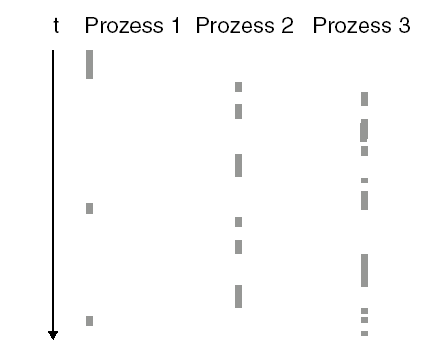
\includegraphics[width=6cm]{images/Concurrency/Quasiparallelitaet.png}
\end{minipage}
\begin{minipage}[c]{10cm}
\begin{itemize}
\item Prozesse/Threads warten die meiste Zeit (blocked).
\item Scheduler ordnet CPU denjenigen Prozessen/Threads zu, die im Zustand ready sind und „'etwas zu tun haben“'
\end{itemize}
\end{minipage}\\\\
Prozesse/Threads können folgende Zustände und Übergänge erfahren:\\
\begin{minipage}[c]{8cm}
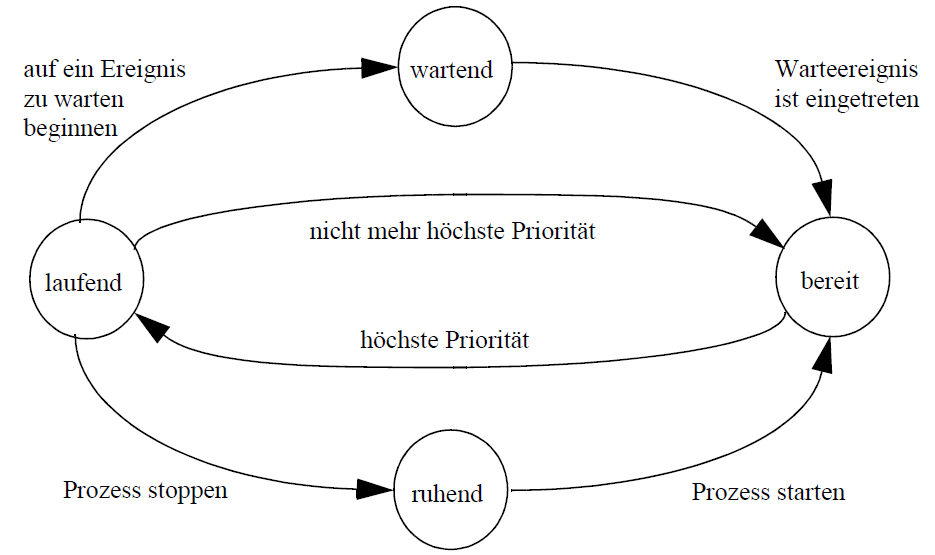
\includegraphics[width=6cm]{images/Concurrency/Prozesszustaende.png}
\end{minipage}
\begin{minipage}[c]{10cm}
\begin{enumerate}
\item I/O Operation, Warten auf Bedingung
\item Scheduler entzieht CPU
\item Scheduler weist CPU zu
\item I/O beendet, Bedingung erfüllt
\end{enumerate}
\end{minipage}

\subsection{Synchonisation: Zugriff auf gemeinsame Ressourcen}
\subsubsection{Kritischer Abschnitt (Critical Section, CS)}
\begin{itemize}
  \item Codebereich, in dem nebenläufige Prozesse oder parallele auf gemeinsame Ressource
  zugreifen. 
  \item Zu jeder Zeit darf sich höchstens ein Prozess im kritischen Bereich
  befinden. 
  \item Der exklusive Zugriff durch höchstens einen Prozess wird mittels gegenseitigem Ausschluss (mutual exclusion, Mutex) sichergestellt. 
\end{itemize}
\subsubsection{Lösungsstruktur für gegenseitigen Ausschluss}
\begin{minipage}[c]{2cm}
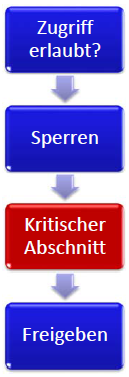
\includegraphics[width=2cm]{images/Concurrency/Loesungsstruktur.png}
\end{minipage}
\begin{minipage}[c]{14cm}
\begin{itemize}
\item Bei der Zugriffsprüfung wird gewartet, bis der Zugang frei wird \\ \ \\ \ \\
\item Beim Sperren wird das Signal auf Rot gesetzt (lock a mutex) \\ \ \\ \ \\ 
\item Beim Freigeben wird das rote Signal wieder gelöscht (unlock a mutex)
\end{itemize}
\end{minipage}
\subsubsection{Forderungen an die Synchronisation (Dijkstra, 1965)}
\begin{enumerate}
  \item Es dürfen sich nicht zwei Prozesse gleichzeitig in ihrem kritischen Abschnitt befinden (mutual exclusion).
  \item Über die Abarbeitungsgeschwindigkeit, bzw. die Anzahl Prozesse dürfen
keine Annahmen getroffen werden. 
  \item Kein Prozess darf ausserhalb eines kritischen Abschnitts einen anderen
Prozess blockieren. 
  \item Jeder Prozess, der am Eingang eines kritischen Abschnitts wartet, muss
irgendwann den Abschnitt betreten dürfen (fairness condition).
\end{enumerate}

\begin{tabbing}
  \hspace*{1cm}\=\hspace*{4.2cm}\=\hspace*{3cm}\=\hspace*{2.7cm}\= \kill
\textbf{Synchro-Versuch 1}\\\\
  \>{\bf Prozess 1} \> \> \>{\bf Prozess 2}\\
  \>\begin{lstlisting}[style=C]
while(grant != 1)
    wait(); 
CS; //Eintritt in Critical Section 
grant = 2; 
    \end{lstlisting} \> \> \>
    \begin{lstlisting}[style=C]
while(grant != 2)
    wait(); 
CS; //Eintritt in Critical Section  
grant = 1; 
    \end{lstlisting} \\\\
    Forderung 2 nicht erfüllt, da sich alle Prozesse selbst daran hindern 2mal nacheinander daran zu kommen.\\\\
    
\textbf{Synchro-Versuch 2}\\\\
   \>{\bf Prozess 1} \> \> \>{\bf Prozess 2}\\
   \>\begin{lstlisting}[style=C]
while(in2)
    wait(); 
in1 = true; 
CS; //Eintritt in Critical Section 
in1 = false; 
    \end{lstlisting} \> \> \>
    \begin{lstlisting}[style=C]
while(in1)
    wait(); 
in2 = true; 
CS; //Eintritt in Critical Section 
in2 = false; 
    \end{lstlisting} \\\\
    Initialisierung ist nicht gelöst.\\\\

\textbf{Synchro-Versuch 3 (Algorithmus von Peterson)}\\\\
   \>{\bf Prozess 1} \> \> \>{\bf Prozess 2}\\
   \>\begin{lstlisting}[style=C]
        request1 = true; 
        grant = 1; 
        while(grant==1 && request2)
          wait(); 
        CS; //Eintritt in Critical Section  
        request1 = false; 
    \end{lstlisting} \> \> \>
    \begin{lstlisting}[style=C]
        request2 = true; 
        grant = 2; 
        while(grant==2 && request1)
          wait(); 
        CS;  //Eintritt in Critical Section 
        request2 = false;  
    \end{lstlisting} \\ 
\end{tabbing}
\vspace*{-1cm}
\textbf{Synchronisation mit Signalen}
\begin{itemize}
  \item Jeder Prozess wartet vor Betreten des kritischen Bereichs auf ein
  gemeinsames Signal. 
  \item Wenn Signal gesetzt $\rightarrow$ kritischer Bereich frei
  \item waitfor(signal) blockiert aufrufenden Prozess, falls signal nicht
  gesetzt
  \item Jeder Prozess, der fertig ist, setzt Signal mit send(signal)
  \item Mehrere Prozesse können gleichzeitig warten 
\end{itemize}

\begin{tabbing}
  \hspace*{1cm}\=\hspace*{4.2cm}\=\hspace*{3cm}\=\hspace*{2.7cm}\= \kill
  \>{\bf Prozess 1} \> \> \>{\bf Prozess 2}\\
  \>\begin{lstlisting}[style=C]
      waitFor(signal); 
      CS;  //Eintritt in Critical Section 
      send(signal); 
    \end{lstlisting} \> \> \>
    \begin{lstlisting}[style=C]
      waitFor(signal); 
      CS;  //Eintritt in Critical Section 
      send(signal); 
    \end{lstlisting} \\\\
 \end{tabbing}
 \vspace*{-1.5cm}
 \subsection{Semaphoren}
 \begin{itemize}
   \item Das Signal für den Zutritt in den kritischen Bereich = Semaphor
   \item Ein Semaphor s hat zwei atomare (= nicht unterbrechbare)
     Operationen
   \begin{itemize}
     \item P(s) : Passieren $\rightarrow$ Beim Eintritt in CS (waitFor)
     \item V(s) : Verlassen $\rightarrow$ Beim Austritt aus CS (send)
   \end{itemize}
   \item Busy waiting
   \begin{itemize}
   \item Beim Busy Waiting warten die Prozesse aktiv in einer Schleife (spin lock)
   \item Wartende Prozesse belasten so unnötigerweise den Prozessor
   \item \textbf{Lösung:} Wartende Prozesse werden in eine Warteschlange eingetragen (sleep und
wakeup)
   \end{itemize}
   \item Probleme bei Semaphoren
   \begin{itemize}
    \item Anwendung erfordert Disziplin
    \begin{itemize}
      \item Für jedes P(s) braucht es auch ein V(s)
      \item Probleme treten auf, wenn V(s) vergessen geht!
    \end{itemize}
    \item In grösseren Programmen können subtile Probleme entstehen, falls z.B. das V(s) in einer if-Bedingung gemacht wird.
    \item Beim Auftreten einer Exception kann das Freigeben ebenfalls
      schwierig sein. 

   \end{itemize}
 \end{itemize}
 
\subsection{Thread-Synchronisation in C mit POSIX Threads}
\lstinputlisting[style=C]{snippets/Concurrency/Sync_POSIX.c}

 \subsubsection{Das Monitorprinzip}
 \begin{itemize}
   \item Grundprinzip: Abstrakten Datenyp (ADT) definieren, der genau die Funktionen
   in der Schnittstelle anbietet, die notwendig sind. 
   \item Der Aufrufer ruft diese Funktionen auf, er muss sich aber nicht um die
   Synchronisation kümmern. 
   \item Die Synchronisation (z.Bsp. mit Semaphoren) ist in der Implementation des
   Monitors lokal gelöst. 
   \item Problem wird einmal im Monitor gelöst, die Aufrufer müssen sich nicht
   mehr darum kümmern. 
 \end{itemize}


\subsection{Petri-Netze}
\subsubsection{Was sind Petri-Netze?}
\begin{itemize}
\item Petri-Netze (Petri Nets) sind eine graphische Darstellung von parallelen Prozessen.
\item Petri-Netze sind bipartite Graphen (Graphen mit zwei Arten von Knoten)
\item Petri-Netze sind mathematische Modelle. Es bestehen Methoden zur
Optimierung und formalen Verifikation (Deadlock-Analyse).
\end{itemize}
\subsubsection{Elemente}
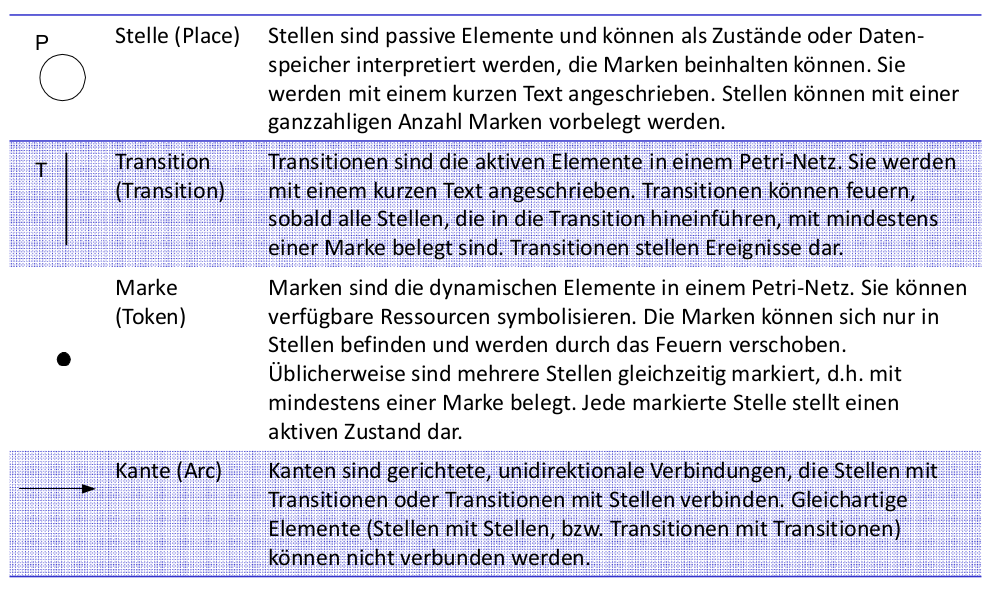
\includegraphics[width=15cm]{images/Concurrency/PetriNetzeElemente}
\newpage
\subsubsection{Feuern von Transitionen}
\begin{itemize}
\item Das Feuern ist die einzige Aktion, die in einem Petri-Netz ausgeführt werden kann.
\item Eine Transition kann dann und nur dann feuern, wenn alle Stellen, die in die Transition hineinführen (Eingabestellen), mit mindestens einer Marke belegt sind. Dann wird bei jeder dieser Stellen eine Marke abgezogen.
\item Jede Stelle, die aus
dieser Transition hinausführt (Ausgabestellen), erhält umgekehrt eine Marke.
\item Das Feuern ist somit das Verschieben von Marken unter definierten Bedingungen.
\end{itemize}
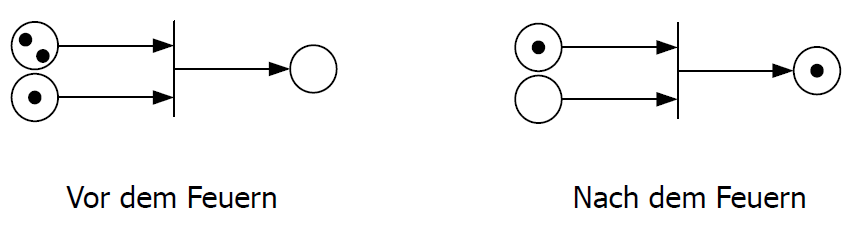
\includegraphics[width=8cm]{images/Concurrency/Petri1}

\begin{description}
  \item[Race Condition]  Das Ergebnis einer Operation hängt von zeitlichen Verhalten bestimmter Einzeloperationen ab.
  \item[Starvation]      Ist ein Zustand, bei dem ein Prozess nie dran kommt (er verhungert). Die Fairness condition besagt, dass Starvation verhindert werden muss.
  \item[Deadlock]        Ist eine Situation in denen sich zwei Prozesse gegenseitig blockieren. Ein Deadlock kann vermieden werden, indem alle Prozesse die gemeinsamen
Ressourcen immer in derselben Reihenfolge anfordern.
\end{description}

\subsubsection{Grundstrukturen}
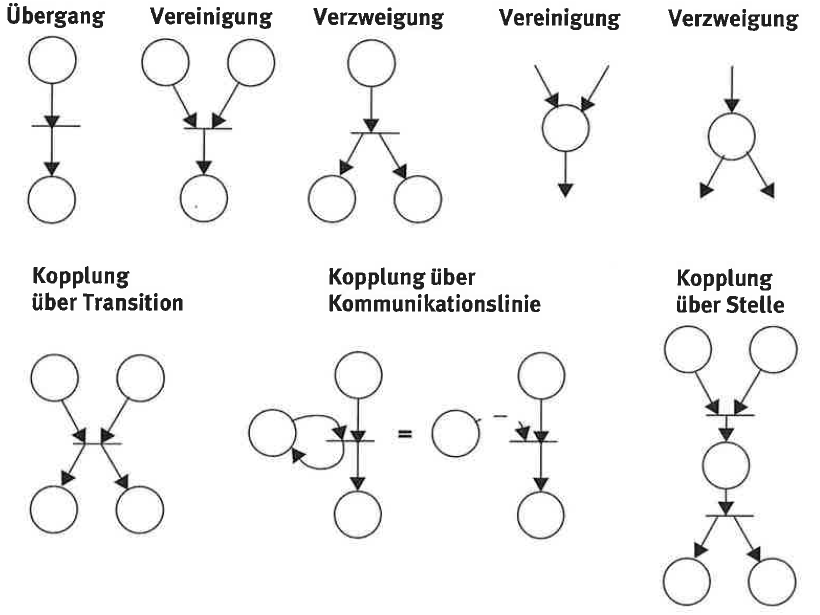
\includegraphics[width=9cm]{images/Concurrency/Petri2}

\vspace*{-1cm}
\subsubsection{Beispiel}
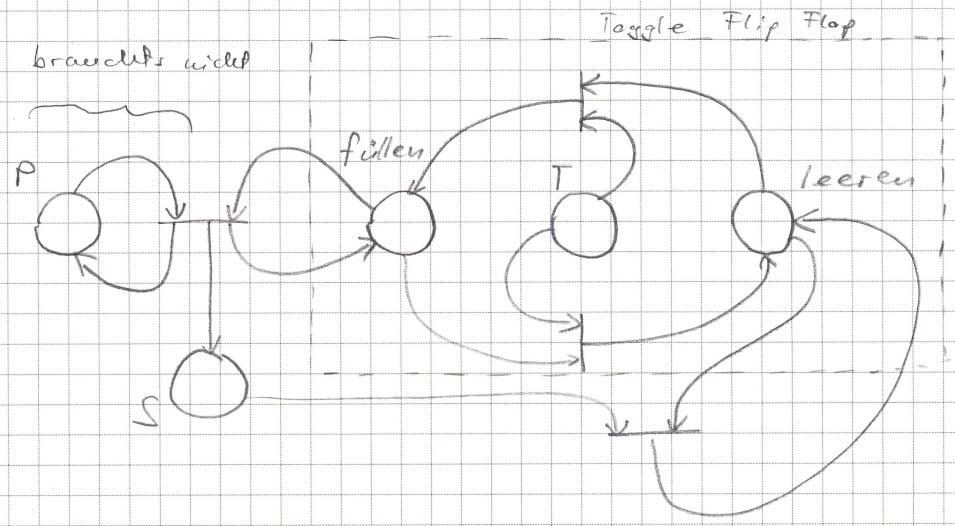
\includegraphics[width=10cm]{images/Concurrency/Petri3}\\
In diesem Beispiel produziert der Produzent P bei jedem Takt ein Marke in S. Sobald eine Marke in T gesetzt wird, wird S geleert. P ist während dieses Vorgangs gesperrt. P produziert wieder, wenn erneut eine Marke in T gesetzt wird. Der Leerprozess wird dann gestoppt.

